\documentclass[11pt]{article}
\usepackage[margin=1in]{geometry}
\usepackage{booktabs}
\usepackage{graphicx}
\usepackage{hyperref}
\usepackage{amsmath}
\usepackage{xcolor}
\usepackage{float}
\usepackage{adjustbox}
\IfFileExists{tables/numbers.tex}{\newcommand{\McpThreeInstances}{109}
\newcommand{\BmRouterFileRecallFiveTwelve}{0.71}
\newcommand{\BmComposedFileRecallTwoK}{0.86}
\newcommand{\BmComposedSymRecallTwoK}{0.41}
\newcommand{\OracleLdtComposedFileRecallTwoK}{0.97}
\newcommand{\BmRouterFileRecallTwoK}{0.72}
\newcommand{\BmRouterSymRecallTwoK}{0.41}
\newcommand{\OracleLdtFileRecallTwoK}{0.96}
\newcommand{\OracleLdtSymRecallTwoK}{0.93}
\newcommand{\BmFilesRecallTwo}{0.07}
\newcommand{\BmFilesTokensTwo}{1733}
\newcommand{\BmFilesRecallFour}{0.18}
\newcommand{\BmFilesTokensFour}{3751}
\newcommand{\BmFilesRecallThirteen}{0.41}
\newcommand{\BmFilesTokensThirteen}{12583}
\newcommand{\BmFilesRecallTwentySeven}{0.53}
\newcommand{\BmFilesTokensTwentySeven}{26568}
\newcommand{\BmMapRecallFive}{0.66}
\newcommand{\BmMapTokensFive}{51}
\newcommand{\BmMapRecallTwelve}{0.76}
\newcommand{\BmMapTokensTwelve}{113}
\newcommand{\BmMapRecallTwentyFive}{0.86}
\newcommand{\BmMapTokensTwentyFive}{231}
\newcommand{\GoldFilesTokens}{9854}
\newcommand{\RepoPythonFiles}{620}
\newcommand{\CompactFirstRouter}{looped\_p4\_d64}
\newcommand{\CompactFirstTokens}{308}
\newcommand{\CompactFirstFileRecall}{0.86}
\newcommand{\CompactSecondRouter}{looped\_p8\_d64}
\newcommand{\CompactSecondTokens}{313}
\newcommand{\CompactSecondFileRecall}{0.84}
\newcommand{\LearnedLocalTokens}{18302}
\newcommand{\BmRouterLocalTokens}{9262}
\newcommand{\BestLearnedRouter}{transformer\_l2\_d64}
\newcommand{\BestLearnedArm}{search}
\newcommand{\BestLearnedFileRecallTwoK}{0.80}
\newcommand{\BestLearnedSymRecallTwoK}{0.22}
\newcommand{\BestLearnedComposedFileRecallTwoK}{0.82}
\newcommand{\BestLearnedComposedSymRecallTwoK}{0.22}
\newcommand{\GdkPacketRuns}{11}
\newcommand{\GdkPacketFileNamed}{5}
\newcommand{\GdkPacketFunctionNamed}{3}
\newcommand{\GdkPacketInputTokens}{2012}
\newcommand{\GdkNoPacketRuns}{11}
\newcommand{\GdkNoPacketFileNamed}{1}
\newcommand{\GdkNoPacketFunctionNamed}{2}
\newcommand{\GdkNoPacketInputTokens}{503}
}{}

\title{Data Goblin: Compact Context Packets from Complex MCP Catalogs\\with Small Looped Routers}
\author{MoralityLab HybridTRMLDT project}
\date{November 2026}

\begin{document}
\maketitle

\begin{abstract}
Frontier coding agents pay per token, while Model Context Protocol (MCP) servers expose catalogs and repositories far
larger than any useful prompt. We study small local routers that explore such MCP surfaces and hand the frontier model
a compact, verifiable context packet. The routers are lexical, dense, feed-forward Transformer, shared-weight looped
Transformer, Tiny Recursive Model (TRM), TRM with certified lattice refinement, and HRM, from about 0.15 to 1.3M
parameters at recurrent depth 1 to 12. The paper reports three measurements:
\begin{itemize}
\item \textbf{Synthetic multi-server catalogs.} Routers with an exact-match token channel solve layered discovery tasks that BM25 and
hand-written rules mostly fail, using about half the tool calls. Looped and recursive cores match a four-layer
Transformer with a quarter of its non-embedding parameters, and deeper recurrence adds nothing measurable.
\item \textbf{SWE-bench Lite.} On \McpThreeInstances{} tasks from ten repositories unseen in training, a 2,048-token
packet that combines a BM25 path map with router-selected source snippets contains the gold files with recall
\BmComposedFileRecallTwoK{} and the gold functions with recall \BmComposedSymRecallTwoK{}. SWE-bench's BM25 whole-file
context reaches \BmFilesRecallTwentySeven{} file recall at \BmFilesTokensTwentySeven{} tokens.
\item \textbf{Cost.} Training a router fits in a few hundred megabytes of process memory, and inference adds megabytes on top of the
runtime.
\end{itemize}
We integrate the packet into Goose as an MCP extension and as a Rust app on the Goose Development Kit. With a local
0.5B model behind the app, the packet raises how often the model names the gold file. Every episode is stored with a
replayable decision tape.

\end{abstract}

\section{Introduction}
A frontier coding agent pays for every token it reads. Model Context Protocol (MCP) servers expose large tool
catalogs, resource hierarchies and code repositories. If the agent explores them directly, it pulls tool schemas, listings and
file contents into its own context. Data Goblin is the intended counterpart: a local retrieval specialist of
about one billion parameters. It spends inexpensive local inference on searching, filtering, cross-referencing and checking,
then hands the frontier agent a compact, verifiable \emph{packet}.

This paper reports the gym built to choose that specialist's architecture, and the first measurements taken with it.
We ask four questions:
\begin{enumerate}
\item Which small router family turns a complex MCP catalog into a correct packet with the fewest tool calls and the
least local compute? The families are lexical BM25, a trained dense dual encoder, feed-forward Transformers,
shared-weight looped Transformers, Tiny Recursive Models (TRM), TRM with certified lattice (LDT) refinement, and a
two-timescale Hierarchical Reasoning Model (HRM).
\item At matched FLOPs, does recurrence with fewer parameters match distinct layers? Does depth added at test time
buy anything?
\item Does a deeper MCP index save more context than its extra traversal costs?
\item On real repositories from a popular code-agent benchmark (SWE-bench Lite), how small can the packet be while
still containing the code the gold patch edits?
\end{enumerate}

Three contributions are executable artifacts in the repository:
\begin{itemize}
\item \textbf{MCP-02}, a synthetic multi-server world with eight compositional task families, layered indices
and candidate refinement certified by an environment-owned verifier.
\item \textbf{MCP-03}, a code-repository MCP over SWE-bench tasks, split by repository.
\item \textbf{goblin-gdk}, a Rust app on the Goose Development Kit (GDK) whose agent loop grounds inference in the packet.
\end{itemize}
Every run stores decision tapes that replay without torch, and continuous integration replays them.


\section{Environments}
\subsection{MCP-02: compositional multi-server catalogs}
Each case is one synthetic organisation served by seven MCP servers with overlapping capabilities: a service
catalog, an org directory, finance, procurement, observability, a replica mirror and an archive. A task names a
service by display name and region. It asks for a value reached through zero to three relation hops (owner team,
cost center, vendor, nested budget section), and may combine two chains by sum or difference. The eight families
each isolate one difficulty:
\begin{itemize}
\item ambiguous names, where a twin service shares the display name in another region;
\item multi-hop joins;
\item arithmetic over two chains;
\item moved records whose old copy is superseded;
\item a catalog epoch change after a hidden number of calls;
\item replica and archive conflicts, including a lexical bait;
\item a value missing from the system of record, which requires abstention;
\item a target placed late in a long paginated collection.
\end{itemize}
Every world also carries confusable names, unit variants, registry entries with unknown metadata (about 12\%), and
unrelated distractors up to the catalog size (256 or 1024 resources).

Splits are grouped. Entity and server names come from disjoint word pools, and each request template belongs
to exactly one split. Only training worlds produce training data. The private judge requires the exact answer, the
abstention flag, and a citation of every required record by a reference issued in the same episode for that
record's current revision.

The four discovery arms share each world. \texttt{flat} returns every descriptor in one call. \texttt{search}
offers paginated BM25. \texttt{layered} walks a facet hierarchy whose layout is a string over server, collection,
record kind, registered provenance, name bucket and entity. \texttt{layered\_ldt} adds explicit per-node
candidate sets bound to the catalog epoch. Every exclusion proposed in that arm passes through
\texttt{certify\_and\_apply\_verified}. Its verifier accepts only when registered metadata proves that every record
below the child serves no record kind the task can cite. Unknown metadata never proves a violation.

\subsection{MCP-03: code-repository MCP on SWE-bench}
Each task is an issue and a repository at the instance's base commit, read from a bare clone. The MCP surface offers:
\begin{itemize}
\item BM25 code search over symbol documents (path, name, signature, docstring and body identifiers);
\item a layered index over directories, modules, classes and methods;
\item symbol reads of at most 80 lines;
\item in the \texttt{layered\_ldt} arm, certified exclusion of subtrees whose every file carries a registered test or
documentation path flag. The public task constraint places edits in library source.
\end{itemize}
The packet is a ranked file map followed by source snippets of the symbols the router read, cut to a budget of
512, 1024, 2048 or 4096 tokens under the pinned Qwen2.5-0.5B-Instruct tokenizer.

Gold targets come from the patch: the changed files, and the innermost function, method or class around each
changed line of the old file. The split is grouped by repository. Training uses 160 django and sympy instances from
SWE-bench minus Lite, and the 32 django and sympy instances from Lite form the dev set. The test set is all 109 SWE-bench Lite
instances from the ten other repositories. The non-agentic reference is SWE-bench's BM25 retrieval: whole files
ranked by BM25 of the issue and packed until the budget.


\section{Router modules and their combinations}
All routers share one observation and one action. The observation holds the open evidence needs and a frontier of
candidate expansions: index branches, result pages, resources or symbols, links, and search queries. In MCP-02 the
needs come from a public plan tracker; in MCP-03 they are the salient code terms of the issue. The action is a score
per candidate, and the loop expands the best one with exactly one MCP tool call. In the LDT arm a router may also
propose exclusions, and the environment certifies each one. When more than 32 non-query candidates are open, the same
BM25 prefilter applies to every router.

\paragraph{Encoder.} Each candidate becomes a hashed word-token sequence \texttt{[CLS] needs [SEP] candidate} (4096
buckets, at most 74 positions), plus a nine-value structural vector: item type, depth, page cursor and log count. The
\texttt{tokens} encoder uses two segment ids. The \texttt{match} encoder also flags tokens that occur in both segments
(segment ids 2 and 3), which is an exact-match channel. It supplies no BM25 score.

\paragraph{Modules.}
\begin{itemize}
\item \textbf{Dense}: a dual encoder with mean-pooled embeddings and MLP towers.
\item \textbf{Transformer}: $L$ distinct pre-LN blocks as a cross-encoder.
\item \textbf{Looped}: one shared block applied $T$ times with a pass embedding.
\item \textbf{TRM}: a shared block updates a latent $z$ from $(x, y, z)$ $n$ times, then the answer state $y$ from
$(y, z)$, repeated for $c$ cycles; the recurrent depth is $c(n+1)$.
\item \textbf{TRM+LDT}: TRM plus an exclusion head whose proposals pass through the certified membrane.
\item \textbf{HRM}: a fast block runs $k$ updates per slow update of a second block, for $h$ slow cycles.
\end{itemize}
The combinations studied are encoder (\texttt{tokens}/\texttt{match}) $\times$ core (distinct, looped, TRM, HRM)
$\times$ LDT (on/off) $\times$ depth (1 to 12 block applications), plus test-time depth changes for the recurrent
cores. Controls are hand-written deterministic rules, BM25, sham random scores, a Transformer trained on shuffled
labels, and an oracle bound that reads private labels.

\paragraph{Training.} Routers imitate oracle labels collected from training worlds. The behaviour policies are the
oracle with no exploration and the oracle with random exploration at $\varepsilon=0.35$. The loss is a listwise softmax
over each state's candidates, with every positive counted. The exclusion head adds a cross-entropy term on certifiable
predicates. Epochs, learning rate and seed are fixed in the configuration; there is no early stopping.


\section{Measurement and economics}
\begin{itemize}
\item \textbf{Retrieval tokens.} The handoff packet is counted three ways:
\begin{itemize}
\item exact UTF-8 bytes;
\item a named tokenizer in MCP-03 (Qwen2.5-0.5B-Instruct, pinned revision);
\item a labelled 4-bytes-per-token estimate in the MCP-02 economics.
\end{itemize}
The tokens the router \emph{read} locally (every tool result) are counted separately, as are router tokens (encoder
positions processed).
\item \textbf{Compute.} FLOPs per candidate come from \texttt{torch.utils.flop\_counter.FlopCounterMode} at the fixed sequence
length, multiplied by the candidates scored. Recurrent depth is the number of block applications. Latency is the
wall clock per router decision on the recorded host.
\item \textbf{Memory.} For training we record the process peak working set, which includes the in-memory dataset, and the CUDA
peak allocation on GPU. For inference we record the peak working-set delta around one 32-candidate forward pass in a
fresh process, together with the weight bytes.
\item \textbf{Economics.} Cost per accepted task divides the summed cost of every assigned episode, failures included, by
the accepted count. The downstream handoff is priced at an assumed frontier input price, and local seconds at
amortised device prices. Tool calls and verifier checks carry nominal prices. All prices are labelled assumptions,
with four sensitivity scenarios.
\end{itemize}
The hosts were shared: an RTX 5080 Laptop GPU with other workloads resident (80 W limit), and a CPU at
full load from concurrent jobs. Wall-clock figures are upper bounds; FLOPs and token counts are host independent.


\section{Results}
\subsection{Compact packets on SWE-bench Lite (MCP-03)}
Table~\ref{tab:mcp03-packets} and Figure~\ref{fig:mcp03} report packet size against localisation on
\McpThreeInstances{} SWE-bench Lite tasks from ten repositories that contributed no training data. A held-out
repository has \RepoPythonFiles{} Python files on average, and its gold files alone average \GoldFilesTokens{}
tokens.

With search access, a router spending 24 local tool calls produces a packet that contains every gold file in a
fraction of tasks no lower than whole-file retrieval at many times the size. BM25 as the router places a gold file in the packet
for a mean file recall of \BmRouterFileRecallFiveTwelve{} at 512 tokens and \BmRouterFileRecallTwoK{} at 2,048
tokens. SWE-bench's BM25 whole-file retrieval reaches \BmFilesRecallTwo{} at 2,048 tokens, \BmFilesRecallThirteen{}
at \BmFilesTokensThirteen{} tokens and \BmFilesRecallTwentySeven{} at \BmFilesTokensTwentySeven{} tokens. Part of the
gap is the packet's ranked path map. Giving the whole-file baseline the same pointer channel (its top 12 BM25 paths,
\BmMapTokensTwelve{} tokens) yields file recall \BmMapRecallTwelve{}. The router's advantage therefore comes from
symbol-level search and reads, not from listing paths.

The oracle bound in the certified LDT arm, which mixes search with index navigation, reaches file recall
\OracleLdtFileRecallTwoK{} and symbol recall \OracleLdtSymRecallTwoK{} at 2,048 tokens, against
\BmRouterSymRecallTwoK{} symbol recall for BM25. That gap is the room a learned router can take. The best learned
router (\texttt{\BestLearnedRouter}, \BestLearnedArm{} arm) reaches file recall \BestLearnedFileRecallTwoK{} and symbol
recall \BestLearnedSymRecallTwoK{}. Without search, browsing the index alone fails for every non-oracle control:
directory names carry too little signal to steer by.

\IfFileExists{tables/mcp03_packets.tex}{\begin{table}[t]
\centering
\small
\begin{adjustbox}{max width=\linewidth}
\begin{tabular}{lrrrrrrrr}
\toprule
Router & Arm & Budget & Packet tok. & File recall & All files & Symbol recall & Calls & Local tok. read \\
\midrule
dense\_d64 & layered +map & 512 & 441.22 & 0.76 & 83/109 & 0.01 & 25.00 & 10106.50 \\
dense\_d64 & layered +map & 2048 & 1506.95 & 0.76 & 83/109 & 0.03 & 25.00 & 10106.50 \\
dense\_d64 & layered & 512 & 444.66 & 0.08 & 9/109 & 0.01 & 25.00 & 10106.50 \\
dense\_d64 & layered & 2048 & 1518.10 & 0.08 & 9/109 & 0.03 & 25.00 & 10106.50 \\
hrm\_h2l1\_d64 & layered +map & 512 & 423.84 & 0.75 & 82/109 & 0.00 & 25.00 & 11401.59 \\
hrm\_h2l1\_d64 & layered +map & 2048 & 1426.52 & 0.75 & 82/109 & 0.02 & 25.00 & 11401.59 \\
hrm\_h2l1\_d64 & layered & 512 & 423.07 & 0.12 & 13/109 & 0.00 & 25.00 & 11401.59 \\
hrm\_h2l1\_d64 & layered & 2048 & 1437.37 & 0.12 & 13/109 & 0.03 & 25.00 & 11401.59 \\
identifier\_rules & layered +map & 512 & 472.19 & 0.75 & 82/109 & 0.02 & 25.00 & 8176.06 \\
identifier\_rules & layered +map & 2048 & 1644.29 & 0.77 & 84/109 & 0.07 & 25.00 & 8176.06 \\
identifier\_rules & layered & 512 & 471.50 & 0.17 & 18/109 & 0.02 & 25.00 & 8176.06 \\
identifier\_rules & layered & 2048 & 1636.88 & 0.17 & 18/109 & 0.07 & 25.00 & 8176.06 \\
lexical\_bm25 & layered +map & 512 & 468.84 & 0.75 & 82/109 & 0.01 & 25.00 & 7692.06 \\
lexical\_bm25 & layered +map & 2048 & 1611.81 & 0.76 & 83/109 & 0.06 & 25.00 & 7692.06 \\
lexical\_bm25 & layered & 512 & 470.02 & 0.07 & 8/109 & 0.01 & 25.00 & 7692.06 \\
lexical\_bm25 & layered & 2048 & 1606.76 & 0.07 & 8/109 & 0.06 & 25.00 & 7692.06 \\
looped\_p4\_d64 & layered +map & 512 & 436.33 & 0.75 & 82/109 & 0.02 & 25.00 & 11738.71 \\
looped\_p4\_d64 & layered +map & 2048 & 1514.69 & 0.75 & 82/109 & 0.06 & 25.00 & 11738.71 \\
looped\_p4\_d64 & layered & 512 & 438.18 & 0.17 & 19/109 & 0.02 & 25.00 & 11738.71 \\
looped\_p4\_d64 & layered & 2048 & 1521.28 & 0.17 & 19/109 & 0.06 & 25.00 & 11738.71 \\
looped\_p8\_d64 & layered +map & 512 & 452.15 & 0.75 & 82/109 & 0.02 & 25.00 & 11614.48 \\
looped\_p8\_d64 & layered +map & 2048 & 1592.13 & 0.75 & 82/109 & 0.03 & 25.00 & 11614.48 \\
looped\_p8\_d64 & layered & 512 & 447.39 & 0.16 & 17/109 & 0.03 & 25.00 & 11614.48 \\
looped\_p8\_d64 & layered & 2048 & 1599.88 & 0.16 & 17/109 & 0.03 & 25.00 & 11614.48 \\
oracle\_upper\_bound & layered +map & 512 & 461.28 & 0.95 & 104/109 & 0.64 & 25.00 & 9836.05 \\
oracle\_upper\_bound & layered +map & 2048 & 1650.79 & 0.95 & 104/109 & 0.89 & 25.00 & 9836.05 \\
oracle\_upper\_bound & layered & 512 & 462.06 & 0.92 & 100/109 & 0.67 & 25.00 & 9836.05 \\
oracle\_upper\_bound & layered & 2048 & 1653.71 & 0.92 & 100/109 & 0.89 & 25.00 & 9836.05 \\
transformer\_l2\_d64 & layered +map & 512 & 415.70 & 0.75 & 82/109 & 0.02 & 25.00 & 11103.33 \\
transformer\_l2\_d64 & layered +map & 2048 & 1452.14 & 0.75 & 82/109 & 0.03 & 25.00 & 11103.33 \\
transformer\_l2\_d64 & layered & 512 & 417.56 & 0.12 & 13/109 & 0.02 & 25.00 & 11103.33 \\
transformer\_l2\_d64 & layered & 2048 & 1450.84 & 0.12 & 13/109 & 0.03 & 25.00 & 11103.33 \\
transformer\_l2\_d64\_tokens & layered +map & 512 & 443.83 & 0.75 & 82/109 & 0.00 & 25.00 & 10851.26 \\
transformer\_l2\_d64\_tokens & layered +map & 2048 & 1661.94 & 0.75 & 82/109 & 0.01 & 25.00 & 10851.26 \\
transformer\_l2\_d64\_tokens & layered & 512 & 444.83 & 0.07 & 8/109 & 0.00 & 25.00 & 10851.26 \\
transformer\_l2\_d64\_tokens & layered & 2048 & 1656.39 & 0.07 & 8/109 & 0.01 & 25.00 & 10851.26 \\
transformer\_l4\_d64 & layered +map & 512 & 430.93 & 0.75 & 82/109 & 0.00 & 25.00 & 10071.64 \\
transformer\_l4\_d64 & layered +map & 2048 & 1232.87 & 0.75 & 82/109 & 0.00 & 25.00 & 10071.64 \\
transformer\_l4\_d64 & layered & 512 & 431.76 & 0.06 & 6/109 & 0.00 & 25.00 & 10071.64 \\
transformer\_l4\_d64 & layered & 2048 & 1248.53 & 0.06 & 6/109 & 0.00 & 25.00 & 10071.64 \\
trm\_c2i1\_d64 & layered +map & 512 & 428.27 & 0.76 & 83/109 & 0.04 & 25.00 & 11456.61 \\
trm\_c2i1\_d64 & layered +map & 2048 & 1506.78 & 0.76 & 83/109 & 0.06 & 25.00 & 11456.61 \\
trm\_c2i1\_d64 & layered & 512 & 430.48 & 0.18 & 20/109 & 0.04 & 25.00 & 11456.61 \\
trm\_c2i1\_d64 & layered & 2048 & 1513.61 & 0.18 & 20/109 & 0.06 & 25.00 & 11456.61 \\
trm\_ldt\_c2i1\_d64 & layered +map & 512 & 440.38 & 0.76 & 83/109 & 0.03 & 25.00 & 11443.83 \\
trm\_ldt\_c2i1\_d64 & layered +map & 2048 & 1627.74 & 0.76 & 83/109 & 0.08 & 25.00 & 11443.83 \\
trm\_ldt\_c2i1\_d64 & layered & 512 & 446.51 & 0.21 & 23/109 & 0.02 & 25.00 & 11443.83 \\
trm\_ldt\_c2i1\_d64 & layered & 2048 & 1628.34 & 0.21 & 23/109 & 0.08 & 25.00 & 11443.83 \\
dense\_d64 & layered\_ldt +map & 512 & 284.31 & 0.76 & 83/109 & 0.04 & 25.00 & 16662.59 \\
dense\_d64 & layered\_ldt +map & 2048 & 694.27 & 0.77 & 84/109 & 0.08 & 25.00 & 16662.59 \\
dense\_d64 & layered\_ldt & 512 & 287.85 & 0.67 & 73/109 & 0.04 & 25.00 & 16662.59 \\
dense\_d64 & layered\_ldt & 2048 & 695.28 & 0.67 & 73/109 & 0.08 & 25.00 & 16662.59 \\
hrm\_h2l1\_d64 & layered\_ldt +map & 512 & 328.28 & 0.78 & 85/109 & 0.07 & 25.00 & 16127.61 \\
hrm\_h2l1\_d64 & layered\_ldt +map & 2048 & 849.63 & 0.78 & 85/109 & 0.12 & 25.00 & 16127.61 \\
hrm\_h2l1\_d64 & layered\_ldt & 512 & 329.28 & 0.68 & 74/109 & 0.08 & 25.00 & 16127.61 \\
hrm\_h2l1\_d64 & layered\_ldt & 2048 & 852.70 & 0.68 & 74/109 & 0.12 & 25.00 & 16127.61 \\
identifier\_rules & layered\_ldt +map & 512 & 489.17 & 0.82 & 89/109 & 0.15 & 25.00 & 9002.02 \\
identifier\_rules & layered\_ldt +map & 2048 & 2010.32 & 0.83 & 91/109 & 0.37 & 25.00 & 9002.02 \\
identifier\_rules & layered\_ldt & 512 & 488.93 & 0.72 & 79/109 & 0.15 & 25.00 & 9002.02 \\
identifier\_rules & layered\_ldt & 2048 & 2010.57 & 0.72 & 79/109 & 0.37 & 25.00 & 9002.02 \\
lexical\_bm25 & layered\_ldt +map & 512 & 487.17 & 0.83 & 91/109 & 0.16 & 25.00 & 9214.20 \\
lexical\_bm25 & layered\_ldt +map & 2048 & 2005.72 & 0.86 & 94/109 & 0.41 & 25.00 & 9214.20 \\
lexical\_bm25 & layered\_ldt & 512 & 489.04 & 0.71 & 77/109 & 0.15 & 25.00 & 9214.20 \\
lexical\_bm25 & layered\_ldt & 2048 & 2007.46 & 0.72 & 78/109 & 0.41 & 25.00 & 9214.20 \\
looped\_p4\_d64 & layered\_ldt +map & 512 & 339.28 & 0.76 & 83/109 & 0.07 & 25.00 & 15466.62 \\
looped\_p4\_d64 & layered\_ldt +map & 2048 & 936.82 & 0.76 & 83/109 & 0.12 & 25.00 & 15466.62 \\
looped\_p4\_d64 & layered\_ldt & 512 & 337.61 & 0.65 & 71/109 & 0.07 & 25.00 & 15466.62 \\
looped\_p4\_d64 & layered\_ldt & 2048 & 939.21 & 0.65 & 71/109 & 0.12 & 25.00 & 15466.62 \\
looped\_p8\_d64 & layered\_ldt +map & 512 & 341.61 & 0.76 & 83/109 & 0.07 & 25.00 & 16167.34 \\
looped\_p8\_d64 & layered\_ldt +map & 2048 & 973.45 & 0.76 & 83/109 & 0.17 & 25.00 & 16167.34 \\
looped\_p8\_d64 & layered\_ldt & 512 & 338.38 & 0.66 & 72/109 & 0.08 & 25.00 & 16167.34 \\
looped\_p8\_d64 & layered\_ldt & 2048 & 978.98 & 0.66 & 72/109 & 0.17 & 25.00 & 16167.34 \\
oracle\_upper\_bound & layered\_ldt +map & 512 & 477.81 & 0.97 & 106/109 & 0.73 & 25.00 & 9924.58 \\
oracle\_upper\_bound & layered\_ldt +map & 2048 & 1951.22 & 0.97 & 106/109 & 0.93 & 25.00 & 9924.58 \\
oracle\_upper\_bound & layered\_ldt & 512 & 479.50 & 0.96 & 105/109 & 0.75 & 25.00 & 9924.58 \\
oracle\_upper\_bound & layered\_ldt & 2048 & 1948.28 & 0.96 & 105/109 & 0.93 & 25.00 & 9924.58 \\
sham\_random & layered\_ldt +map & 512 & 485.71 & 0.76 & 83/109 & 0.06 & 25.00 & 9191.49 \\
sham\_random & layered\_ldt +map & 2048 & 1876.75 & 0.80 & 87/109 & 0.21 & 25.00 & 9191.49 \\
sham\_random & layered\_ldt & 512 & 484.60 & 0.56 & 61/109 & 0.06 & 25.00 & 9191.49 \\
sham\_random & layered\_ldt & 2048 & 1881.06 & 0.56 & 61/109 & 0.22 & 25.00 & 9191.49 \\
transformer\_l2\_d64 & layered\_ldt +map & 512 & 372.06 & 0.78 & 85/109 & 0.06 & 25.00 & 15146.77 \\
transformer\_l2\_d64 & layered\_ldt +map & 2048 & 1133.17 & 0.78 & 85/109 & 0.11 & 25.00 & 15146.77 \\
transformer\_l2\_d64 & layered\_ldt & 512 & 371.94 & 0.56 & 61/109 & 0.06 & 25.00 & 15146.77 \\
transformer\_l2\_d64 & layered\_ldt & 2048 & 1137.06 & 0.56 & 61/109 & 0.11 & 25.00 & 15146.77 \\
transformer\_l2\_d64\_tokens & layered\_ldt +map & 512 & 344.01 & 0.76 & 83/109 & 0.07 & 25.00 & 15957.29 \\
transformer\_l2\_d64\_tokens & layered\_ldt +map & 2048 & 987.62 & 0.77 & 84/109 & 0.10 & 25.00 & 15957.29 \\
transformer\_l2\_d64\_tokens & layered\_ldt & 512 & 337.43 & 0.61 & 67/109 & 0.07 & 25.00 & 15957.29 \\
transformer\_l2\_d64\_tokens & layered\_ldt & 2048 & 991.50 & 0.61 & 67/109 & 0.10 & 25.00 & 15957.29 \\
transformer\_l4\_d64 & layered\_ldt +map & 512 & 346.01 & 0.78 & 85/109 & 0.07 & 25.00 & 16347.61 \\
transformer\_l4\_d64 & layered\_ldt +map & 2048 & 917.57 & 0.78 & 85/109 & 0.15 & 25.00 & 16347.61 \\
transformer\_l4\_d64 & layered\_ldt & 512 & 342.63 & 0.71 & 77/109 & 0.07 & 25.00 & 16347.61 \\
transformer\_l4\_d64 & layered\_ldt & 2048 & 920.17 & 0.71 & 77/109 & 0.15 & 25.00 & 16347.61 \\
trm\_c2i1\_d64 & layered\_ldt +map & 512 & 263.49 & 0.75 & 82/109 & 0.08 & 25.00 & 17070.45 \\
trm\_c2i1\_d64 & layered\_ldt +map & 2048 & 627.06 & 0.75 & 82/109 & 0.13 & 25.00 & 17070.45 \\
trm\_c2i1\_d64 & layered\_ldt & 512 & 260.54 & 0.74 & 81/109 & 0.08 & 25.00 & 17070.45 \\
trm\_c2i1\_d64 & layered\_ldt & 2048 & 631.17 & 0.74 & 81/109 & 0.13 & 25.00 & 17070.45 \\
trm\_ldt\_c2i1\_d64 & layered\_ldt +map & 512 & 260.74 & 0.77 & 84/109 & 0.06 & 25.00 & 17106.02 \\
trm\_ldt\_c2i1\_d64 & layered\_ldt +map & 2048 & 600.57 & 0.77 & 84/109 & 0.09 & 25.00 & 17106.02 \\
trm\_ldt\_c2i1\_d64 & layered\_ldt & 512 & 266.72 & 0.72 & 78/109 & 0.06 & 25.00 & 17106.02 \\
trm\_ldt\_c2i1\_d64 & layered\_ldt & 2048 & 597.84 & 0.72 & 78/109 & 0.09 & 25.00 & 17106.02 \\
dense\_d64 & search +map & 512 & 262.54 & 0.76 & 83/109 & 0.06 & 25.00 & 18335.23 \\
dense\_d64 & search +map & 2048 & 543.30 & 0.77 & 84/109 & 0.10 & 25.00 & 18335.23 \\
dense\_d64 & search & 512 & 266.34 & 0.78 & 85/109 & 0.06 & 25.00 & 18335.23 \\
dense\_d64 & search & 2048 & 546.70 & 0.78 & 85/109 & 0.10 & 25.00 & 18335.23 \\
hrm\_h2l1\_d64 & search +map & 512 & 301.28 & 0.78 & 85/109 & 0.08 & 25.00 & 18203.50 \\
hrm\_h2l1\_d64 & search +map & 2048 & 754.83 & 0.78 & 85/109 & 0.15 & 25.00 & 18203.50 \\
hrm\_h2l1\_d64 & search & 512 & 303.94 & 0.83 & 91/109 & 0.10 & 25.00 & 18203.50 \\
hrm\_h2l1\_d64 & search & 2048 & 758.69 & 0.83 & 91/109 & 0.15 & 25.00 & 18203.50 \\
identifier\_rules & search +map & 512 & 489.17 & 0.82 & 89/109 & 0.15 & 25.00 & 9016.83 \\
identifier\_rules & search +map & 2048 & 2010.32 & 0.83 & 91/109 & 0.37 & 25.00 & 9016.83 \\
identifier\_rules & search & 512 & 488.61 & 0.72 & 79/109 & 0.15 & 25.00 & 9016.83 \\
identifier\_rules & search & 2048 & 2010.79 & 0.72 & 79/109 & 0.37 & 25.00 & 9016.83 \\
lexical\_bm25 & search +map & 512 & 488.96 & 0.83 & 91/109 & 0.16 & 25.00 & 9262.32 \\
lexical\_bm25 & search +map & 2048 & 2016.54 & 0.86 & 94/109 & 0.41 & 25.00 & 9262.32 \\
lexical\_bm25 & search & 512 & 490.04 & 0.71 & 77/109 & 0.15 & 25.00 & 9262.32 \\
lexical\_bm25 & search & 2048 & 2018.03 & 0.72 & 79/109 & 0.41 & 25.00 & 9262.32 \\
looped\_p4\_d64 & search +map & 512 & 303.50 & 0.78 & 85/109 & 0.10 & 25.00 & 18421.38 \\
looped\_p4\_d64 & search +map & 2048 & 727.65 & 0.79 & 86/109 & 0.18 & 25.00 & 18421.38 \\
looped\_p4\_d64 & search & 512 & 307.55 & 0.86 & 94/109 & 0.11 & 25.00 & 18421.38 \\
looped\_p4\_d64 & search & 2048 & 729.76 & 0.86 & 94/109 & 0.18 & 25.00 & 18421.38 \\
looped\_p8\_d64 & search +map & 512 & 314.05 & 0.76 & 83/109 & 0.08 & 25.00 & 18198.09 \\
looped\_p8\_d64 & search +map & 2048 & 837.72 & 0.78 & 85/109 & 0.20 & 25.00 & 18198.09 \\
looped\_p8\_d64 & search & 512 & 313.05 & 0.84 & 92/109 & 0.09 & 25.00 & 18198.09 \\
looped\_p8\_d64 & search & 2048 & 842.13 & 0.84 & 92/109 & 0.20 & 25.00 & 18198.09 \\
oracle\_upper\_bound & search +map & 512 & 485.19 & 0.87 & 95/109 & 0.47 & 25.00 & 9517.60 \\
oracle\_upper\_bound & search +map & 2048 & 2019.17 & 0.87 & 95/109 & 0.62 & 25.00 & 9517.60 \\
oracle\_upper\_bound & search & 512 & 485.47 & 0.73 & 80/109 & 0.49 & 25.00 & 9517.60 \\
oracle\_upper\_bound & search & 2048 & 2017.20 & 0.74 & 81/109 & 0.62 & 25.00 & 9517.60 \\
sham\_random & search +map & 512 & 487.48 & 0.80 & 87/109 & 0.08 & 25.00 & 9832.14 \\
sham\_random & search +map & 2048 & 2002.82 & 0.83 & 90/109 & 0.24 & 25.00 & 9832.14 \\
sham\_random & search & 512 & 487.20 & 0.62 & 68/109 & 0.08 & 25.00 & 9832.14 \\
sham\_random & search & 2048 & 1999.10 & 0.64 & 70/109 & 0.24 & 25.00 & 9832.14 \\
transformer\_l2\_d64 & search +map & 512 & 340.53 & 0.80 & 87/109 & 0.10 & 25.00 & 18008.17 \\
transformer\_l2\_d64 & search +map & 2048 & 934.65 & 0.82 & 89/109 & 0.22 & 25.00 & 18008.17 \\
transformer\_l2\_d64 & search & 512 & 346.41 & 0.80 & 87/109 & 0.10 & 25.00 & 18008.17 \\
transformer\_l2\_d64 & search & 2048 & 936.27 & 0.80 & 87/109 & 0.22 & 25.00 & 18008.17 \\
transformer\_l2\_d64\_tokens & search +map & 512 & 327.96 & 0.76 & 83/109 & 0.07 & 25.00 & 17368.54 \\
transformer\_l2\_d64\_tokens & search +map & 2048 & 893.36 & 0.77 & 84/109 & 0.12 & 25.00 & 17368.54 \\
transformer\_l2\_d64\_tokens & search & 512 & 324.58 & 0.72 & 78/109 & 0.07 & 25.00 & 17368.54 \\
transformer\_l2\_d64\_tokens & search & 2048 & 899.14 & 0.72 & 78/109 & 0.12 & 25.00 & 17368.54 \\
transformer\_l4\_d64 & search +map & 512 & 326.86 & 0.78 & 85/109 & 0.10 & 25.00 & 18120.25 \\
transformer\_l4\_d64 & search +map & 2048 & 830.78 & 0.78 & 85/109 & 0.19 & 25.00 & 18120.25 \\
transformer\_l4\_d64 & search & 512 & 326.48 & 0.78 & 85/109 & 0.10 & 25.00 & 18120.25 \\
transformer\_l4\_d64 & search & 2048 & 834.51 & 0.78 & 85/109 & 0.19 & 25.00 & 18120.25 \\
trm\_c2i1\_d64 & search +map & 512 & 241.47 & 0.75 & 82/109 & 0.08 & 25.00 & 18579.46 \\
trm\_c2i1\_d64 & search +map & 2048 & 451.42 & 0.75 & 82/109 & 0.13 & 25.00 & 18579.46 \\
trm\_c2i1\_d64 & search & 512 & 237.24 & 0.84 & 92/109 & 0.08 & 25.00 & 18579.46 \\
trm\_c2i1\_d64 & search & 2048 & 457.16 & 0.84 & 92/109 & 0.13 & 25.00 & 18579.46 \\
trm\_ldt\_c2i1\_d64 & search +map & 512 & 239.56 & 0.77 & 84/109 & 0.05 & 25.00 & 18553.39 \\
trm\_ldt\_c2i1\_d64 & search +map & 2048 & 493.93 & 0.78 & 85/109 & 0.08 & 25.00 & 18553.39 \\
trm\_ldt\_c2i1\_d64 & search & 512 & 246.49 & 0.83 & 90/109 & 0.05 & 25.00 & 18553.39 \\
trm\_ldt\_c2i1\_d64 & search & 2048 & 499.21 & 0.83 & 90/109 & 0.08 & 25.00 & 18553.39 \\
bm25\_whole\_files & direct & 2048 & 1733.17 & 0.07 & 8/109 & -- & 0 & -- \\
bm25\_whole\_files & direct & 4096 & 3750.83 & 0.18 & 20/109 & -- & 0 & -- \\
bm25\_whole\_files & direct & 13000 & 12582.98 & 0.41 & 45/109 & -- & 0 & -- \\
bm25\_whole\_files & direct & 27000 & 26567.86 & 0.53 & 58/109 & -- & 0 & -- \\
bm25\_path\_map\_top5 & direct & -- & 50.95 & 0.66 & 72/109 & -- & 0 & -- \\
bm25\_path\_map\_top12 & direct & -- & 113.30 & 0.76 & 83/109 & -- & 0 & -- \\
bm25\_path\_map\_top25 & direct & -- & 230.64 & 0.86 & 94/109 & -- & 0 & -- \\
\bottomrule
\end{tabular}
\end{adjustbox}
\caption{MCP-03 on 109 SWE-bench Lite instances from ten repositories unseen in training: packet size (Qwen2.5 tokenizer) against localisation of the gold patch, with the tokens the router read locally.}
\label{tab:mcp03-packets}
\end{table}
}{}
\IfFileExists{figures/mcp03_tokens_vs_recall.pdf}{
\begin{figure}[t]\centering
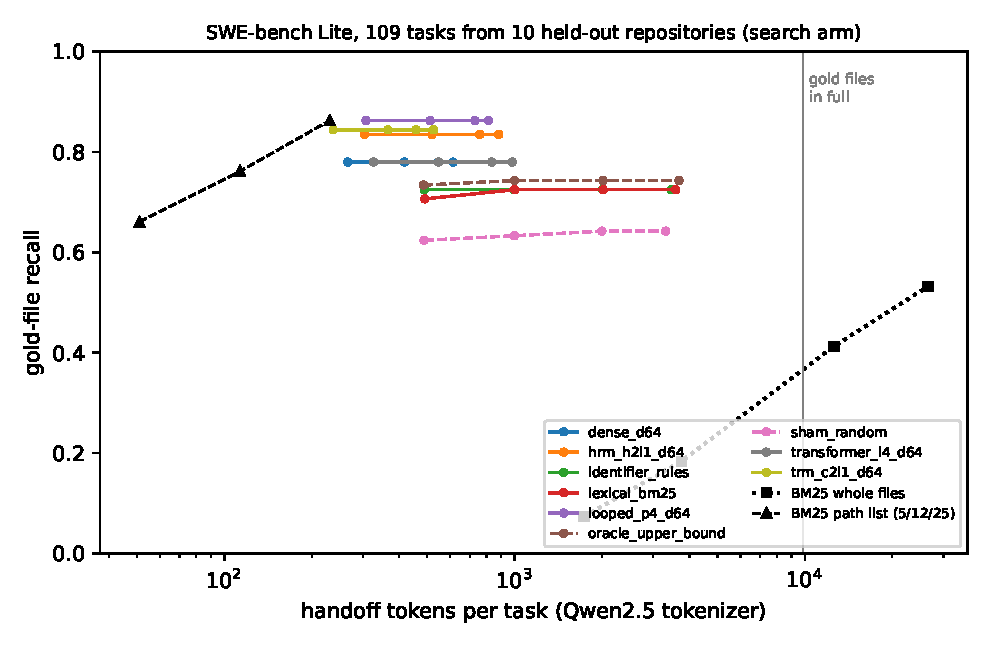
\includegraphics[width=0.85\linewidth]{figures/mcp03_tokens_vs_recall.pdf}
\caption{Handoff tokens against gold-file recall on held-out SWE-bench Lite repositories.}\label{fig:mcp03}
\end{figure}}{}

\IfFileExists{sections/results_mcp02.tex}{\subsection{Synthetic multi-server catalogs (MCP-02)}
\paragraph{Index depth.} At 1024 resources the layout sweep (Table~\ref{tab:mcp02-pilot_gpu-layout},
Figure~\ref{fig:layout}) separates three regimes:
\begin{itemize}
\item paging a flat root or a single server facet exhausts the 40-call budget even for the oracle;
\item two facets are not enough either;
\item three or four facets (server, collection and name bucket, or kind, bucket and entity) let the oracle finish in
14 to 20 calls while reading about half the tool-result bytes of a shallow walk.
\end{itemize}
Deeper indices therefore pay for their traversal once the catalog no longer fits a few pages per node.
Certified exclusions cost refine calls but prune whole provenance or capability subtrees. With the provenance
facet first they remove archive and replica branches in one step, and no certified exclusion ever removed a
required record.

\paragraph{Controls.} Search and eager flat listing are easy for BM25 and the deterministic rules at both catalog
sizes. Layered discovery without search is hard: at 1024 resources both controls solve only a few episodes per cell,
while the oracle solves nearly all of them. That gap is where learned routing can matter.

\paragraph{Learned routers.} Tables~\ref{tab:mcp02-pilot_cpu-success} and \ref{tab:mcp02-pilot_gpu-success} give
accepted episodes per cell for the CPU pilot (width 48, tokens-only encoder) and the GPU pilot (width 128, exact-match
channel). The encoder dominates. Tokens-only routers stay below BM25 in most cells, because they never learn to
recognise that a candidate's identifier equals the needed one. Adding the exact-match channel lifts held-out dev
ranking accuracy from 0.73 to 0.91 for the same Transformer-L2 and data, and it is what lets learned routers compete.
Among tokens-only routers the TRM is the strongest learned family in the layered arms, consistent with recurrence
helping when matching must be learned.

\IfFileExists{tables/mcp02_pilot_gpu_success.tex}{\begin{table}[t]
\centering
\small
\begin{adjustbox}{max width=\linewidth}
\begin{tabular}{lcccccccccc}
\toprule
Router & flat@256 & layered/KBE@256 & layered/SCB@256 & layered\_ldt/PSCB@256 & search@256 & flat@1024 & layered/KBE@1024 & layered/SCB@1024 & layered\_ldt/PSCB@1024 & search@1024 \\
\midrule
dense\_d128 & 32/32 & 28/32 & 24/32 & 22/32 & 32/32 & 32/32 & 7/32 & 5/32 & 5/32 & 32/32 \\
deterministic\_rules & 32/32 & 22/32 & 12/32 & 10/32 & 32/32 & 32/32 & 2/32 & 5/32 & 3/32 & 32/32 \\
hrm\_h2l1\_d128 & 32/32 & 30/32 & 30/32 & 27/32 & 32/32 & 32/32 & 17/32 & 10/32 & 5/32 & 31/32 \\
lexical\_bm25 & 32/32 & 22/32 & 11/32 & 7/32 & 32/32 & 32/32 & 6/32 & 1/32 & 1/32 & 32/32 \\
looped\_p12\_d128 & 32/32 & 31/32 & 28/32 & 27/32 & 32/32 & 32/32 & 20/32 & 11/32 & 8/32 & 31/32 \\
looped\_p4\_d128 & 32/32 & 32/32 & 29/32 & 27/32 & 32/32 & 32/32 & 18/32 & 13/32 & 10/32 & 31/32 \\
oracle\_upper\_bound & 32/32 & 32/32 & 32/32 & 32/32 & 32/32 & 32/32 & 26/32 & 31/32 & 31/32 & 32/32 \\
sham\_random & 10/32 & 0/32 & 1/32 & 0/32 & 27/32 & 8/32 & 0/32 & 0/32 & 0/32 & 21/32 \\
sham\_shuffled\_transformer\_l2\_d128 & 0/32 & 0/32 & 0/32 & 0/32 & 11/32 & 0/32 & 0/32 & 0/32 & 0/32 & 11/32 \\
transformer\_l1\_d128 & 32/32 & 29/32 & 30/32 & 26/32 & 32/32 & 32/32 & 19/32 & 10/32 & 7/32 & 31/32 \\
transformer\_l2\_d128 & 32/32 & 32/32 & 28/32 & 25/32 & 32/32 & 32/32 & 22/32 & 9/32 & 6/32 & 31/32 \\
transformer\_l2\_d128\_tokens & 26/32 & 24/32 & 16/32 & 8/32 & 32/32 & 20/32 & 9/32 & 1/32 & 0/32 & 27/32 \\
transformer\_l4\_d128 & 32/32 & 31/32 & 30/32 & 27/32 & 32/32 & 32/32 & 23/32 & 14/32 & 9/32 & 31/32 \\
trm\_c2i1\_d128 & 32/32 & 30/32 & 31/32 & 28/32 & 32/32 & 32/32 & 15/32 & 10/32 & 5/32 & 31/32 \\
trm\_c4i2\_d128 & 32/32 & 30/32 & 30/32 & 26/32 & 32/32 & 32/32 & 14/32 & 9/32 & 4/32 & 31/32 \\
trm\_ldt\_c2i1\_d128 & 32/32 & 32/32 & 32/32 & 27/32 & 32/32 & 32/32 & 20/32 & 8/32 & 6/32 & 31/32 \\
\bottomrule
\end{tabular}
\end{adjustbox}
\caption{MCP-02 pilot gpu: accepted episodes per arm and catalog size (32 held-out test worlds per cell, 40-call budget).}
\label{tab:mcp02-pilot_gpu-success}
\end{table}
}{}
\IfFileExists{tables/mcp02_pilot_cpu_success.tex}{\begin{table}[t]
\centering
\small
\begin{adjustbox}{max width=\linewidth}
\begin{tabular}{lcccccccccc}
\toprule
Router & flat@256 & layered/KBE@256 & layered/SCB@256 & layered\_ldt/PSCB@256 & search@256 & flat@1024 & layered/KBE@1024 & layered/SCB@1024 & layered\_ldt/PSCB@1024 & search@1024 \\
\midrule
dense\_d48 & 17/32 & 1/32 & 1/32 & 2/32 & 30/32 & 11/32 & 0/32 & 0/32 & 0/32 & 29/32 \\
deterministic\_rules & 32/32 & 22/32 & 12/32 & 10/32 & 32/32 & 32/32 & 2/32 & 5/32 & 3/32 & 32/32 \\
hrm\_h2l1\_d48 & 18/32 & 16/32 & 6/32 & 3/32 & 28/32 & 9/32 & 6/32 & 0/32 & 0/32 & 20/32 \\
lexical\_bm25 & 32/32 & 22/32 & 11/32 & 7/32 & 32/32 & 32/32 & 6/32 & 1/32 & 1/32 & 32/32 \\
looped\_p4\_d48 & 16/32 & 11/32 & 5/32 & 4/32 & 30/32 & 13/32 & 8/32 & 0/32 & 0/32 & 24/32 \\
oracle\_upper\_bound & 32/32 & 32/32 & 32/32 & 32/32 & 32/32 & 32/32 & 26/32 & 31/32 & 31/32 & 32/32 \\
sham\_random & 10/32 & 0/32 & 1/32 & 0/32 & 27/32 & 8/32 & 0/32 & 0/32 & 0/32 & 21/32 \\
sham\_shuffled\_transformer\_l2\_d48 & 1/32 & 1/32 & 0/32 & 0/32 & 21/32 & 2/32 & 0/32 & 0/32 & 0/32 & 21/32 \\
transformer\_l1\_d48 & 16/32 & 13/32 & 4/32 & 3/32 & 28/32 & 7/32 & 3/32 & 0/32 & 0/32 & 21/32 \\
transformer\_l2\_d48 & 16/32 & 17/32 & 4/32 & 5/32 & 30/32 & 8/32 & 5/32 & 1/32 & 0/32 & 19/32 \\
transformer\_l2\_d48\_match & 32/32 & 31/32 & 29/32 & 26/32 & 32/32 & 32/32 & 16/32 & 9/32 & 6/32 & 31/32 \\
transformer\_l4\_d48 & 19/32 & 17/32 & 6/32 & 4/32 & 26/32 & 12/32 & 8/32 & 0/32 & 0/32 & 26/32 \\
trm\_c2i1\_d48 & 18/32 & 20/32 & 7/32 & 5/32 & 27/32 & 10/32 & 2/32 & 0/32 & 0/32 & 23/32 \\
trm\_c2i1\_d48\_match & 32/32 & 30/32 & 29/32 & 28/32 & 32/32 & 32/32 & 20/32 & 12/32 & 3/32 & 28/32 \\
trm\_ldt\_c2i1\_d48 & 18/32 & 17/32 & 5/32 & 3/32 & 31/32 & 10/32 & 1/32 & 0/32 & 0/32 & 21/32 \\
\bottomrule
\end{tabular}
\end{adjustbox}
\caption{MCP-02 pilot cpu: accepted episodes per arm and catalog size (32 held-out test worlds per cell, 40-call budget).}
\label{tab:mcp02-pilot_cpu-success}
\end{table}
}{}
\IfFileExists{tables/mcp02_pilot_gpu_depth.tex}{\begin{table}[t]
\centering
\small
\begin{adjustbox}{max width=\linewidth}
\begin{tabular}{lrrrrr}
\toprule
Router & Arm & Test depth & Accepted & Calls/ep & GFLOPs/ep \\
\midrule
hrm\_h2l1\_d128 & layered/SCB & 1 & 30/32 & 18.28 & 26.06 \\
hrm\_h2l1\_d128 & layered/SCB & 2 & 30/32 & 18.34 & 52.32 \\
hrm\_h2l1\_d128 & layered/SCB & 4 & 30/32 & 18.47 & 105.19 \\
hrm\_h2l1\_d128 & layered/SCB & 8 & 30/32 & 18.41 & 209.26 \\
hrm\_h2l1\_d128 & layered\_ldt/PSCB & 1 & 25/32 & 26.62 & 29.94 \\
hrm\_h2l1\_d128 & layered\_ldt/PSCB & 2 & 27/32 & 25.12 & 56.33 \\
hrm\_h2l1\_d128 & layered\_ldt/PSCB & 4 & 27/32 & 25.41 & 115.21 \\
hrm\_h2l1\_d128 & layered\_ldt/PSCB & 8 & 27/32 & 25.56 & 232.96 \\
looped\_p4\_d128 & layered/SCB & 1 & 25/32 & 25.31 & 20.32 \\
looped\_p4\_d128 & layered/SCB & 2 & 27/32 & 22.84 & 36.25 \\
looped\_p4\_d128 & layered/SCB & 4 & 29/32 & 19.06 & 54.79 \\
looped\_p4\_d128 & layered/SCB & 8 & 30/32 & 18.31 & 101.94 \\
looped\_p4\_d128 & layered\_ldt/PSCB & 1 & 19/32 & 31.72 & 20.35 \\
looped\_p4\_d128 & layered\_ldt/PSCB & 2 & 25/32 & 28.75 & 37.83 \\
looped\_p4\_d128 & layered\_ldt/PSCB & 4 & 27/32 & 24.84 & 55.22 \\
looped\_p4\_d128 & layered\_ldt/PSCB & 8 & 28/32 & 25.44 & 106.32 \\
trm\_c2i1\_d128 & layered/SCB & 1 & 31/32 & 18.19 & 25.50 \\
trm\_c2i1\_d128 & layered/SCB & 2 & 31/32 & 18.47 & 52.14 \\
trm\_c2i1\_d128 & layered/SCB & 4 & 31/32 & 17.81 & 99.10 \\
trm\_c2i1\_d128 & layered/SCB & 8 & 31/32 & 17.81 & 198.08 \\
trm\_c2i1\_d128 & layered\_ldt/PSCB & 1 & 27/32 & 25.72 & 28.09 \\
trm\_c2i1\_d128 & layered\_ldt/PSCB & 2 & 28/32 & 25.34 & 53.95 \\
trm\_c2i1\_d128 & layered\_ldt/PSCB & 4 & 28/32 & 25.34 & 108.52 \\
trm\_c2i1\_d128 & layered\_ldt/PSCB & 8 & 28/32 & 25.25 & 215.54 \\
trm\_ldt\_c2i1\_d128 & layered/SCB & 1 & 31/32 & 17.94 & 24.88 \\
trm\_ldt\_c2i1\_d128 & layered/SCB & 2 & 32/32 & 16.88 & 45.53 \\
trm\_ldt\_c2i1\_d128 & layered/SCB & 4 & 32/32 & 16.81 & 90.47 \\
trm\_ldt\_c2i1\_d128 & layered/SCB & 8 & 32/32 & 16.84 & 181.47 \\
trm\_ldt\_c2i1\_d128 & layered\_ldt/PSCB & 1 & 27/32 & 26.56 & 32.32 \\
trm\_ldt\_c2i1\_d128 & layered\_ldt/PSCB & 2 & 27/32 & 25.59 & 61.92 \\
trm\_ldt\_c2i1\_d128 & layered\_ldt/PSCB & 4 & 28/32 & 24.75 & 119.49 \\
trm\_ldt\_c2i1\_d128 & layered\_ldt/PSCB & 8 & 28/32 & 24.69 & 240.16 \\
\bottomrule
\end{tabular}
\end{adjustbox}
\caption{Recurrent depth changed at test time only (trained depth in the router name).}
\label{tab:mcp02-pilot_gpu-depth}
\end{table}
}{}
\IfFileExists{tables/mcp02_pilot_gpu_layout.tex}{\begin{table}[t]
\centering
\small
\begin{adjustbox}{max width=\linewidth}
\begin{tabular}{lrrrrrrr}
\toprule
Router & Arm & Layout & Depth & Accepted & Calls/ep & Result KB/ep & Certified excl. \\
\midrule
deterministic\_rules & layered & - & 1 & 0/16 & 40.00 & 82.60 & 0 \\
deterministic\_rules & layered & S & 2 & 0/16 & 40.00 & 111.37 & 0 \\
deterministic\_rules & layered & SC & 3 & 0/16 & 40.00 & 79.23 & 0 \\
deterministic\_rules & layered & KBE & 4 & 0/16 & 40.00 & 103.58 & 0 \\
deterministic\_rules & layered & KSB & 4 & 1/16 & 38.06 & 85.82 & 0 \\
deterministic\_rules & layered & SCB & 4 & 3/16 & 34.94 & 81.71 & 0 \\
deterministic\_rules & layered & PKBE & 5 & 1/16 & 38.94 & 94.73 & 0 \\
deterministic\_rules & layered & PSCB & 5 & 1/16 & 38.75 & 130.26 & 0 \\
deterministic\_rules & layered\_ldt & - & 1 & 0/16 & 40.00 & 111.89 & 1292 \\
deterministic\_rules & layered\_ldt & S & 2 & 0/16 & 40.00 & 103.49 & 700 \\
deterministic\_rules & layered\_ldt & SC & 3 & 0/16 & 40.00 & 79.41 & 5 \\
deterministic\_rules & layered\_ldt & KBE & 4 & 5/16 & 38.00 & 92.45 & 85 \\
deterministic\_rules & layered\_ldt & KSB & 4 & 1/16 & 38.25 & 77.62 & 96 \\
deterministic\_rules & layered\_ldt & SCB & 4 & 3/16 & 35.12 & 80.09 & 141 \\
deterministic\_rules & layered\_ldt & PKBE & 5 & 1/16 & 38.81 & 79.05 & 92 \\
deterministic\_rules & layered\_ldt & PSCB & 5 & 1/16 & 38.75 & 103.28 & 92 \\
oracle\_upper\_bound & layered & - & 1 & 0/16 & 40.00 & 83.64 & 0 \\
oracle\_upper\_bound & layered & S & 2 & 1/16 & 39.06 & 103.91 & 0 \\
oracle\_upper\_bound & layered & SC & 3 & 6/16 & 30.44 & 80.67 & 0 \\
oracle\_upper\_bound & layered & KBE & 4 & 14/16 & 16.56 & 38.79 & 0 \\
oracle\_upper\_bound & layered & KSB & 4 & 13/16 & 20.31 & 64.14 & 0 \\
oracle\_upper\_bound & layered & SCB & 4 & 15/16 & 14.06 & 40.86 & 0 \\
oracle\_upper\_bound & layered & PKBE & 5 & 13/16 & 19.50 & 38.60 & 0 \\
oracle\_upper\_bound & layered & PSCB & 5 & 10/16 & 23.94 & 49.16 & 0 \\
oracle\_upper\_bound & layered\_ldt & - & 1 & 0/16 & 40.00 & 116.96 & 1292 \\
oracle\_upper\_bound & layered\_ldt & S & 2 & 1/16 & 39.06 & 109.34 & 467 \\
oracle\_upper\_bound & layered\_ldt & SC & 3 & 5/16 & 31.50 & 82.82 & 48 \\
oracle\_upper\_bound & layered\_ldt & KBE & 4 & 15/16 & 19.19 & 40.13 & 97 \\
oracle\_upper\_bound & layered\_ldt & KSB & 4 & 14/16 & 20.62 & 59.78 & 96 \\
oracle\_upper\_bound & layered\_ldt & SCB & 4 & 15/16 & 15.69 & 44.02 & 7 \\
oracle\_upper\_bound & layered\_ldt & PKBE & 5 & 14/16 & 21.69 & 39.73 & 153 \\
oracle\_upper\_bound & layered\_ldt & PSCB & 5 & 15/16 & 20.56 & 46.15 & 158 \\
trm\_c2i1\_d128 & layered & - & 1 & 0/16 & 40.00 & 84.12 & 0 \\
trm\_c2i1\_d128 & layered & S & 2 & 1/16 & 39.06 & 128.38 & 0 \\
trm\_c2i1\_d128 & layered & SC & 3 & 1/16 & 38.50 & 130.15 & 0 \\
trm\_c2i1\_d128 & layered & KBE & 4 & 8/16 & 34.56 & 76.22 & 0 \\
trm\_c2i1\_d128 & layered & KSB & 4 & 7/16 & 34.12 & 128.74 & 0 \\
trm\_c2i1\_d128 & layered & SCB & 4 & 6/16 & 33.75 & 107.08 & 0 \\
trm\_c2i1\_d128 & layered & PKBE & 5 & 4/16 & 35.12 & 72.11 & 0 \\
trm\_c2i1\_d128 & layered & PSCB & 5 & 2/16 & 36.75 & 106.22 & 0 \\
trm\_c2i1\_d128 & layered\_ldt & - & 1 & 0/16 & 40.00 & 116.95 & 1292 \\
trm\_c2i1\_d128 & layered\_ldt & S & 2 & 1/16 & 39.06 & 112.60 & 565 \\
trm\_c2i1\_d128 & layered\_ldt & SC & 3 & 1/16 & 38.56 & 138.73 & 526 \\
trm\_c2i1\_d128 & layered\_ldt & KBE & 4 & 6/16 & 35.31 & 76.15 & 88 \\
trm\_c2i1\_d128 & layered\_ldt & KSB & 4 & 7/16 & 35.25 & 127.07 & 93 \\
trm\_c2i1\_d128 & layered\_ldt & SCB & 4 & 6/16 & 34.12 & 105.65 & 102 \\
trm\_c2i1\_d128 & layered\_ldt & PKBE & 5 & 5/16 & 36.25 & 70.03 & 122 \\
trm\_c2i1\_d128 & layered\_ldt & PSCB & 5 & 3/16 & 37.06 & 105.20 & 115 \\
trm\_ldt\_c2i1\_d128 & layered & - & 1 & 0/16 & 40.00 & 84.13 & 0 \\
trm\_ldt\_c2i1\_d128 & layered & S & 2 & 0/16 & 40.00 & 145.81 & 0 \\
trm\_ldt\_c2i1\_d128 & layered & SC & 3 & 2/16 & 36.62 & 124.36 & 0 \\
trm\_ldt\_c2i1\_d128 & layered & KBE & 4 & 10/16 & 33.00 & 73.03 & 0 \\
trm\_ldt\_c2i1\_d128 & layered & KSB & 4 & 5/16 & 35.19 & 135.66 & 0 \\
trm\_ldt\_c2i1\_d128 & layered & SCB & 4 & 5/16 & 32.62 & 110.71 & 0 \\
trm\_ldt\_c2i1\_d128 & layered & PKBE & 5 & 4/16 & 36.81 & 74.51 & 0 \\
trm\_ldt\_c2i1\_d128 & layered & PSCB & 5 & 4/16 & 34.00 & 97.48 & 0 \\
trm\_ldt\_c2i1\_d128 & layered\_ldt & - & 1 & 0/16 & 40.00 & 90.18 & 243 \\
trm\_ldt\_c2i1\_d128 & layered\_ldt & S & 2 & 0/16 & 40.00 & 132.92 & 208 \\
trm\_ldt\_c2i1\_d128 & layered\_ldt & SC & 3 & 2/16 & 36.81 & 124.50 & 17 \\
trm\_ldt\_c2i1\_d128 & layered\_ldt & KBE & 4 & 4/16 & 36.62 & 67.21 & 54 \\
trm\_ldt\_c2i1\_d128 & layered\_ldt & KSB & 4 & 4/16 & 35.50 & 134.13 & 59 \\
trm\_ldt\_c2i1\_d128 & layered\_ldt & SCB & 4 & 6/16 & 32.94 & 110.87 & 4 \\
trm\_ldt\_c2i1\_d128 & layered\_ldt & PKBE & 5 & 1/16 & 39.00 & 62.86 & 98 \\
trm\_ldt\_c2i1\_d128 & layered\_ldt & PSCB & 5 & 4/16 & 35.31 & 99.94 & 122 \\
\bottomrule
\end{tabular}
\end{adjustbox}
\caption{Index layout and depth at 1024 resources: deeper facet hierarchies against traversal cost.}
\label{tab:mcp02-pilot_gpu-layout}
\end{table}
}{}
\IfFileExists{figures/mcp02_layout_depth.pdf}{
\begin{figure}[t]\centering
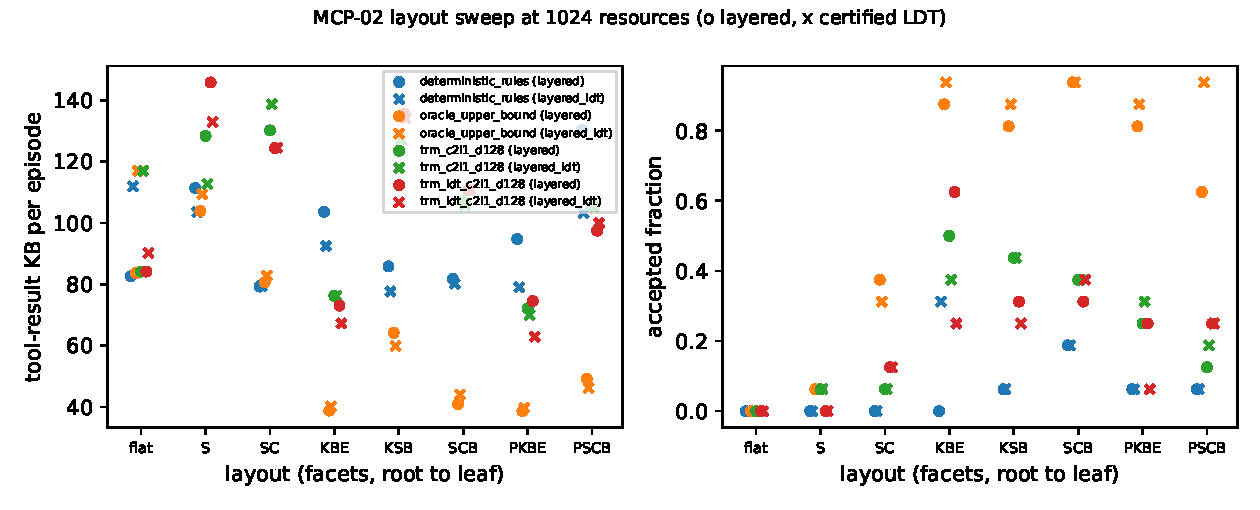
\includegraphics[width=0.95\linewidth]{figures/mcp02_layout_depth.pdf}
\caption{MCP-02 index depth against tool-result volume and accepted episodes (1024 resources).}\label{fig:layout}
\end{figure}}{}
}{}
\IfFileExists{sections/results_resources.tex}{\subsection{Compute and memory of the router modules}
Tables~\ref{tab:mcp03-receipts}, \ref{tab:mcp02-pilot_gpu-receipts} and \ref{tab:mcp02-pilot_cpu-receipts} list, per module:
\begin{itemize}
\item measured parameters (total and without the hashed embedding);
\item recurrent depth in block applications;
\item FLOPs per scored candidate;
\item router latency per decision;
\item peak memory for training and inference.
\end{itemize}
All modules are small: the hashed embedding dominates the parameter count, and a scored decision costs
megaFLOPs to low gigaFLOPs. Recurrence trades parameters for FLOPs. At equal depth, a looped block or a TRM
holds the parameters of one block but pays the FLOPs of four, while the four-layer Transformer pays both.
Training memory is dominated by the framework runtime and the in-memory dataset rather than by the router. The
inference forward adds a few megabytes on top of the runtime.

\IfFileExists{tables/mcp03_receipts.tex}{\begin{table}[t]
\centering
\small
\begin{adjustbox}{max width=\linewidth}
\begin{tabular}{lrrrrrrrrrrrr}
\toprule
Router & Family & Params & Non-emb. & Depth & FLOPs/cand. & ms/dec. & Infer +MiB & Train CPU +MiB & Train CUDA MiB & s/step GPU & File R@2K+map & Sym R@2K \\
\midrule
dense\_d64 & dense & 301633 & 38977 & 0 & 66688 & 18.69 & 3 & 129 & 44 & 0.46 & 0.77 & 0.08 \\
hrm\_h2l1\_d64 & hrm & 368577 & 105921 & 4 & 34706688 & 162.09 & 23 & 756 & 645 & 0.49 & 0.78 & 0.12 \\
looped\_p4\_d64 & looped & 320513 & 57857 & 4 & 34706688 & 165.14 & 22 & 740 & 637 & 0.59 & 0.76 & 0.12 \\
looped\_p8\_d64 & looped & 320513 & 57857 & 8 & 69412096 & 308.11 & 22 & 1317 & 1204 & 0.96 & 0.76 & 0.17 \\
transformer\_l2\_d64 & transformer & 368449 & 105793 & 2 & 17353984 & 87.96 & 21 & 452 & 343 & 0.48 & 0.78 & 0.11 \\
transformer\_l2\_d64\_tokens & transformer & 368321 & 105665 & 2 & 17353984 & 85.20 & 20 & 452 & 343 & 0.47 & 0.77 & 0.10 \\
transformer\_l4\_d64 & transformer & 468417 & 205761 & 4 & 34706688 & 167.68 & 22 & 744 & 628 & 0.57 & 0.78 & 0.15 \\
trm\_c2i1\_d64 & trm & 318593 & 55937 & 4 & 34706688 & 167.06 & 22 & 740 & 644 & 0.52 & 0.75 & 0.13 \\
trm\_ldt\_c2i1\_d64 & trm\_ldt & 318918 & 56262 & 4 & 34707328 & 166.11 & 23 & 792 & 711 & 0.58 & 0.77 & 0.09 \\
\bottomrule
\end{tabular}
\end{adjustbox}
\caption{MCP-03 router modules: measured size, recurrent depth, FLOPs per candidate, latency, inference memory delta around a 32-candidate forward, training memory over 15 CPU / 40 GPU steps (CPU: growth above the loaded dataset and runtime; GPU: peak allocation), and held-out localisation in the LDT arm.}
\label{tab:mcp03-receipts}
\end{table}
}{}
\IfFileExists{tables/mcp02_pilot_gpu_receipts.tex}{\begin{table}[t]
\centering
\small
\begin{adjustbox}{max width=\linewidth}
\begin{tabular}{lrrrrrrrrrr}
\toprule
Router & Family & Params & Non-emb. & Depth & FLOPs/cand. & ms/decision & Infer RSS MiB & Train RSS MiB & Train CUDA MiB & Dev top-1 \\
\midrule
dense\_d128 & dense & 668801 & 143489 & 0 & 264448 & 15.54 & 358.10 & -- & -- & 0.84 \\
hrm\_h2l1\_d128 & hrm & 933761 & 408449 & 16 & 510429696 & 34.77 & 426.00 & 2470 & 927 & 0.92 \\
looped\_p12\_d128 & looped & 739329 & 214017 & 12 & 382822912 & 66.98 & 427.30 & 2446 & 2579 & 0.91 \\
looped\_p4\_d128 & looped & 739329 & 214017 & 4 & 127609344 & 36.22 & 427.90 & -- & 913 & 0.91 \\
sham\_shuffled\_transformer\_l2\_d128 & transformer & 933505 & 408193 & 2 & 63805952 & 20.84 & 427.30 & 2478 & 507 & 0.14 \\
transformer\_l1\_d128 & transformer & 735233 & 209921 & 1 & 31904256 & 15.91 & 427.10 & -- & -- & 0.91 \\
transformer\_l2\_d128 & transformer & 933505 & 408193 & 2 & 63805952 & 21.57 & 426.90 & -- & -- & 0.91 \\
transformer\_l2\_d128\_tokens & transformer & 933249 & 407937 & 2 & 63805952 & 21.69 & 427.60 & -- & -- & 0.73 \\
transformer\_l4\_d128 & transformer & 1330049 & 804737 & 4 & 127609344 & 30.53 & 427.00 & -- & -- & 0.91 \\
trm\_c2i1\_d128 & trm & 735489 & 210177 & 4 & 127609344 & 38.14 & 427.50 & -- & 924 & 0.91 \\
trm\_c4i2\_d128 & trm & 735489 & 210177 & 12 & 382822912 & 67.73 & 429.30 & 2458 & 2595 & 0.91 \\
trm\_ldt\_c2i1\_d128 & trm\_ldt & 736134 & 210822 & 4 & 127610624 & 37.38 & 427.40 & 2498 & 922 & 0.90 \\
\bottomrule
\end{tabular}
\end{adjustbox}
\caption{MCP-02 pilot gpu router receipts: measured parameters, recurrent depth (block applications), FLOPs per candidate (FlopCounterMode), router latency, peak memory.}
\label{tab:mcp02-pilot_gpu-receipts}
\end{table}
}{}
\IfFileExists{tables/mcp02_pilot_cpu_receipts.tex}{\begin{table}[t]
\centering
\small
\begin{adjustbox}{max width=\linewidth}
\begin{tabular}{lrrrrrrrrrr}
\toprule
Router & Family & Params & Non-emb. & Depth & FLOPs/cand. & ms/decision & Infer RSS MiB & Train RSS MiB & Train CUDA MiB & Dev top-1 \\
\midrule
dense\_d48 & dense & 219985 & 22993 & 0 & 37728 & 22.54 & 3.30 & -- & -- & 0.48 \\
hrm\_h2l1\_d48 & hrm & 257905 & 60913 & 16 & 82293696 & 96.33 & 22.00 & 1482 & -- & 0.61 \\
looped\_p4\_d48 & looped & 231073 & 34081 & 4 & 20574144 & 96.91 & 20.60 & -- & -- & 0.56 \\
sham\_shuffled\_transformer\_l2\_d48 & transformer & 257809 & 60817 & 2 & 10287552 & 49.17 & 20.90 & 1313 & -- & 0.16 \\
transformer\_l1\_d48 & transformer & 229537 & 32545 & 1 & 5144256 & 49.61 & 19.00 & -- & -- & 0.56 \\
transformer\_l2\_d48 & transformer & 257809 & 60817 & 2 & 10287552 & 81.31 & 20.60 & -- & -- & 0.62 \\
transformer\_l2\_d48\_match & transformer & 257905 & 60913 & 2 & 10287552 & 49.30 & 20.30 & 1290 & -- & 0.88 \\
transformer\_l4\_d48 & transformer & 314353 & 117361 & 4 & 20574144 & 84.70 & 20.90 & -- & -- & 0.65 \\
trm\_c2i1\_d48 & trm & 229633 & 32641 & 4 & 20574144 & 366.54 & 21.30 & -- & -- & 0.61 \\
trm\_c2i1\_d48\_match & trm & 229729 & 32737 & 4 & 20574144 & 107.48 & 22.10 & 1512 & -- & 0.86 \\
trm\_ldt\_c2i1\_d48 & trm\_ldt & 229878 & 32886 & 4 & 20574624 & 100.19 & 22.10 & 1483 & -- & 0.61 \\
\bottomrule
\end{tabular}
\end{adjustbox}
\caption{MCP-02 pilot cpu router receipts: measured parameters, recurrent depth (block applications), FLOPs per candidate (FlopCounterMode), router latency, peak memory.}
\label{tab:mcp02-pilot_cpu-receipts}
\end{table}
}{}
}{}


\section{Goose integration}
The packet reaches a Goose agent in two ways.

\paragraph{MCP extension.} \texttt{MCP/mcp03/goblin\_server.py} is an MCP stdio server with two tools:
\begin{itemize}
\item \texttt{compact\_context(task, repo\_path, budget\_tokens, max\_tool\_calls, arm)} runs a router over a live
working tree and returns the packet with its accounting: packet tokens, tokens read locally, tool calls, router FLOPs.
\item \texttt{read\_symbol} returns one symbol's source.
\end{itemize}
Goose loads it as an extension with \texttt{--with-extension}.

\paragraph{GDK app.} \texttt{goblin-gdk} is a Rust binary on \texttt{goose-agent} and \texttt{goose-providers}
0.1.0-alpha.14, the Goose Development Kit's agent loop and provider layer. Its state machine has two steps:
\begin{enumerate}
\item \texttt{CompactContextOperation}, a GDK \texttt{Operation}, contributes the goblin packet as the prompt part
\texttt{retrieved\_code\_context}. The machine collects it into the next inference request.
\item \texttt{InferenceRunner} calls an OpenAI-compatible endpoint through \texttt{OpenAiCompatibleProvider}.
\end{enumerate}
The app talks to the goblin server over MCP stdio JSON-RPC. With \texttt{--no-packet} it runs the same machine
without the operation's contribution. Provider-reported token usage is recorded through a custom
\texttt{InferenceEffect}. Continuous integration builds the app and checks it against a scripted endpoint: the packet
must appear in the provider request, stay within its budget, and be smaller than what the router read.
Table~\ref{tab:gdk-demo} reports a run with a real local model: Qwen2.5-0.5B-Instruct on CPU, asked to name the
file and function to edit for SWE-bench Lite tasks from three held-out repositories.
\begin{itemize}
\item With the 1.5K-token packet it named a gold file in \GdkPacketFileNamed{} of \GdkPacketRuns{} tasks and a gold
function in \GdkPacketFunctionNamed{}, at \GdkPacketInputTokens{} provider input tokens per task.
\item Without the packet it managed \GdkNoPacketFileNamed{} and \GdkNoPacketFunctionNamed{}, at \GdkNoPacketInputTokens{}
tokens.
\end{itemize}
The sample is small and the model weak, so this shows the integration path rather than a frontier-scale effect.

\IfFileExists{tables/gdk_demo.tex}{\begin{table}[t]
\centering
\small
\begin{adjustbox}{max width=\linewidth}
\begin{tabular}{lrrrrrrr}
\toprule
Run & Tasks & Packet tok. & Provider in & Provider out & File named & Function named & Inference s \\
\midrule
with goblin packet & 11 & 1508.82 & 2012.27 & 128.73 & 5 & 3 & 374.52 \\
without packet & 11 & -- & 503.45 & 107.91 & 1 & 2 & 307.08 \\
\bottomrule
\end{tabular}
\end{adjustbox}
\caption{goblin-gdk with Qwen2.5-0.5B-Instruct on CPU: SWE-bench Lite tasks from requests, flask and seaborn. The model must name the file and function to edit; answers are scored against the hidden gold patch.}
\label{tab:gdk-demo}
\end{table}
}{}


\section{Limitations}
\begin{itemize}
\item \textbf{Synthetic worlds.} MCP-02 tasks are generated. Their exact judge makes accounting precise, but descriptor
language and catalog structure are simpler than real MCP deployments.
\item \textbf{Localisation, not resolution.} MCP-03 measures whether the packet contains the code the gold patch
edits. That is the retrieval stage of agentless SWE-bench pipelines. We did not measure an end-to-end resolve rate. No frontier-model API
key was available on the host, and the local model that fit beside the other resident workloads (Qwen2.5-0.5B) could
not even drive the synthetic controller task (Table~\ref{tab:llm-controllers}). The GDK demo therefore scores whether
that model names the gold file and function, on 11 tasks, not whether a patch passes the tests.
\item \textbf{Small training budgets.} Routers saw at most tens of thousands of decision states for two or three epochs.
Architecture differences of a few points are within noise at 32 to 109 tasks per cell. The paper reports Wilson
intervals and paired bootstrap intervals rather than significance claims.
\item \textbf{Shared hardware.} The GPU and CPU served concurrent jobs, so latencies are upper bounds and comparisons
across runs taken at different times are not exact. FLOPs, tokens and memory peaks are not affected.
\item \textbf{Encoder amendment.} The exact-match channel was added after inspecting dev-world decision traces of a
tokens-only router, and before any test-set evaluation of a learned router. The CPU pilot keeps the registered tokens-only
encoder for comparison.
\end{itemize}


\section{Next experiment and Data Goblin objective}
\paragraph{Data Goblin as a training objective.} The measurements above select the gym's
interface for a specialist of about one billion parameters. Its parts:
\begin{itemize}
\item \textbf{Inputs.} The public task, the MCP surface or a candidate frontier, read results, and the explicit candidate
state of a layered index.
\item \textbf{Outputs.} One MCP action per step (an expansion, a certified-exclusion proposal, or the final packet). Packets cite
environment-issued references within a strict byte budget.
\item \textbf{Supervision.} First, imitation of oracle-routed trajectories from repository-grouped training data, with failed routes
kept and labelled. Then policy optimisation against the exact judge, with reward equal to negative failure-inclusive
cost per accepted task under a hard downstream context budget.
\item \textbf{Deliberation.} Local tool calls, recurrent depth and generated tokens are free variables whose compute is
counted. None of it reaches the frontier model except through the packet.
\item \textbf{Certification.} Hard exclusions only through \texttt{certify\_and\_apply\_verified}. Learned relevance stays soft.
\end{itemize}

\IfFileExists{sections/next_experiment.tex}{\paragraph{Next experiment.} The experiment with the highest expected information gain is a \emph{read-aware} router on
MCP-03, evaluated on the same 109 held-out tasks. The learned routers already rank files better than BM25 in a quarter
of the tokens, but they read too few symbols. The oracle shows that 24 calls are enough to place most gold
functions in a 2K-token packet.

The design:
\begin{itemize}
\item Keep the best file-ranking core (the four-pass looped block or the TRM; both cheap) for the exploration phase.
\item Label states on-policy, with DAgger-style relabelling of the router's own trajectories, instead of only the oracle's.
\item Add a packet-level objective: symbol recall within the token budget, charged for every local call.
\end{itemize}

The decisive measurement is whether gold-symbol recall at 1K tokens exceeds BM25's 0.41 at 2K tokens while file
recall stays at or above 0.85. If it does, the next step is a downstream run in which a frontier model receives only
the packet and its resource handles, and resolves the SWE-bench tasks. That run turns token savings into measured
cost per resolved issue.

For the synthetic catalogs, the matching experiment trains on mixed catalog sizes (256 and 1024). It would test
whether the four-fold size drop seen here is a training-distribution effect or a capacity limit of 0.2M-parameter
cores.
}{}


\appendix
\section{Reproduction}
The code is in \texttt{MCP/mcp02}, \texttt{MCP/mcp03} and \texttt{MCP/goose\_gdk\_app} of the HybridTRMLDT repository,
on branch \texttt{gym/mcp-local-retrieval-20261119}. Configurations are in \texttt{MCP/mcp02/configs} and
\texttt{MCP/mcp03/configs}.

Result directories under \texttt{MCP/results} hold:
\begin{itemize}
\item compressed episode records;
\item decision tapes (observation digest, chosen index, normalised scores, cost);
\item model receipts (parameters, FLOPs per candidate, checkpoint SHA-256, training receipt with peak memory);
\item host and source manifests.
\end{itemize}
\texttt{python -m MCP.mcp02.run replay} and \texttt{python -m MCP.mcp03.run replay} re-execute episodes from their tapes
without torch, and the CI workflow \texttt{mcp-gym.yml} does so on every push. Checkpoints stay outside Git; their
hashes identify them.

\texttt{goose-gdk-app.yml} builds the GDK app and runs \texttt{ci\_smoke.py} against a scripted OpenAI-compatible
endpoint. The tables in this paper are produced by \texttt{papers/mcp\_data\_goblin/make\_tables.py} from those files.


\end{document}
